%\section{Defining disaggregation}
\section{Formalisms}
\label{sec:problem}

%Different research efforts define the problem of energy disaggregation
%in different ways.

Since Hart first defined the problem of energy disaggregation~\cite{hart1992}, its
exact definition has varied slightly. To make the problem more tractable and to
tailor it to specific use cases, researchers have made varying assumptions
about what information is given.
The bare bones version of disaggregation, as originally proposed
by Hart~\cite{hart1992}, assumes that only
aggregated current and voltage data is available as features. Other
researchers assume additional information is known, such as, 
the total number of devices\footnote{Disaggregation can only be meaningfully
  performed for devices/appliances whose power consumption is over a minimal
  threshold, typically 50 to 200 W. The number of devices here refer to those above this
  threshold.}, the number of steady power consumption states of 
devices and their corresponding power levels, and non AC power features. 
There are thus numerous formulations of the energy disaggregation problem and
these distinctions need to be considered while performances of
algorithms are compared. 
Broadly, the disaggregation problem can be solved in supervised,
unsupervised, or semi-supervised settings.

%\subsection{Definition of Supervised Energy Disaggregation}
In supervised learning approaches, labeled data is available for a period of
time, i.e., the on/off state of each device is known. 
For instance, \cite{liang2010load} assume that all devices are known
and formulate the objective function as one of 
minimizing error between the disaggregated devices and 
the corresponding ground truth devices. 
In~\cite{kolter2012aistat} it is
assumed that the power levels of individual devices are known. 
The problem then is to find the on/off events
for different devices over a period of time.
The input to supervised learning methods is thus training data consisting of
aggregated power and non-power features over time T, and each device's power
consumption over T.
Once a model is trained, given new data over
time T', the output is the disaggregated power for each device over T'.
In addition to 
power related features such as current, voltage, 
or the non-powers features such as time of day, day of week, month season,
weather information, may be given. 

\iffalse
Unsupervised or semi-supervised energy disaggregation is a harder problem since 
labeled data is not available, including any information regarding power
levels of devices. Some researchers assume the
number of devices or circuits (see Section x for details) are
known~\cite{kim2010unsupervised,kolter2012aistat,parson2012nonintrusive,johnson2012bayesian,shao2013temporal}.
\manishc{can you add a few more refs to this}
\huijuanc{change as following paragraph}.
This information can typically be found from circuit wiring diagrams.
Others assume no
such information, e.g.,~\cite{gonccalves2011unsupervised}
and~\cite{wytock2014contextually}, 
\manishc{is the accuracy of these methods (which assume no information at all
  low? Here you want to provide a high level comparison between the
  unsupervised/supervised approaches} \huijuanc{agree. The follows is the revised paragraph}
 \fi 
Unsupervised or semi-supervised energy disaggregation is a harder problem because, 
comparing to supervised learning approaches, the only known information is the aggregated 
data. 
The number of devices/circuits or the characteristics of each device, 
such as power levels are either unknown~\cite{gonccalves2011unsupervised,wytock2014contextually}
or assumed by the researchers to be fixed~\cite{kim2011unsupervised,kolter2012aistat,parson2012nonintrusive,johnson2012bayesian,shao2013temporal}.  
In spite of these difficulties, the
disaggregation performance of unsupervised approaches 
may approach that of supervised approaches. 
%
%In particular, it is assumed that 
%the detailed devices information is unavailable, 
%such as the number of power levels (the steady states of a device), 
% the power value of each level, and the 
%exact time when it is turned on or off. 
Note that evaluation of any method, whether supervised or unsupervised, requires that
ground truth information be available (number of devices and their on/off power states).

%In the evaluation phase, 
%even if we do not know the number of devices,
%we still need to compare the disaggregated 
%devices with the true devices. 
%Therefore we assume the number of devices is known. 

%\textit{Energy Disaggregation with Power}
%Given the aggregated power record $Y=y_1, ..., y_i, ..., y_T$
%in the unit of watts
%over a period of time $T$, 
%the ground truth of $N$ time series 
%$X_j = x_{1j}, ...x_{ij}, ... x_{Tj}, j\in[1, N]$ 
%corresponding to $N$ circuits or devices, 
%estimate disaggregated $N$ time series 
%$\hat{X_j }= \hat{x_{1j}}, ...\hat{x_{ij}}, ... \hat{x_{Tj}}, j\in[1, N]$, 
%such that 
%the L2 norm error between the disaggregated power values and 
%the ground truth is minimal as in equation \ref{eq_powerObj}.
%\begin{equation}
%\label{eq_powerObj}
%\min_{\hat{x_{ij}}} \sum_{i=1}^T (\sum_{j=1}^N \hat{x_{ij}}-y_i)^2
%\end{equation}
%For supervised learning, we know each time series, 
%then equation \ref{eq_powerObj} can be written as 
%$\min_{\hat{x_{ij}}} \sum_{i=1}^T \sum_{j=1}^N (\hat{x_{ij}} - x_{ij})^2$ 
%for L2 norm. 

\subsection{Definition}
For our purposes, we will assume the following definition of the problem:
Given an aggregate power consumption time series $Y=y_1, ..., y_T$, and a set of
power related and contextual features, $f=f_1, ..., f_T$ over a period of time T, 
the problem is to estimate the disaggregated power consumption of $M$ devices 
$\hat{X_m }= \hat{x}_{1}^{(m)}, ...\hat{x}_{t}^{(m)}, ... \hat{x}_{T}^{(m)}, m\in[1, M]$, 
such that a loss function on the sum of the power consumption of the $M$
devices and the aggregate power consumption is minimal. 
\begin{equation}
\label{eq_powerObj}
\min_{\hat{x}_{t}^{(m)}} \{ \sum_{t=1}^T \mathscr{L}_t(\sum_{m=1}^M \hat{x}_{t}^{(m)}, y_t) \}
\end{equation}
where $\mathscr{L}_t$ is the loss function between 
the sum of $M$ estimated time series at $t$, 
and $y_t$ is the ground truth aggregated power feature at time $t$. 
$\mathscr{L}$ is usually the $\mathscr{L}1$-norm $\sum_{m=1}^M |\hat{x}_{t}^{(m)} - y_t|$
or the $\mathscr{L}2$-norm $\sum_{m=1}^M (\hat{x}_{t}^{(m)}-y_t)^2$.

For supervised learning, 
the ground truth of $M$ time series 
$X_m = x_{1}^{(m)}, ...x_{t}^{(m)}, ... x_{T}^{(m)}, m\in[1, M]$ 
corresponding to $M$ circuits or devices is also given.
%Equation (\ref{eq_powerObj}) is written as 
%$\min_{\hat{x}_{t}^{(m)}} \{ \mathscr{L}_{t}^{(m)}(\sum_{t=1}^T \sum_{m=1}^M \hat{x}_{t}^{(m)}, y_t) \}$.
%\manishc{pushing the sum over T into the loss function is not correct; also y
%  still depends on t} \huijuanc{already deleted.}

%% Given a set of time series $Y=y_1, ..., y_T$, 
%% the aggregated power feature over a period of time T, 
%% and contextual features of $M$ devices; 
%% the problem is to estimate disaggregated $M$ time series 
%% $\hat{X_m }= \hat{x}_{1}^{(m)}, ...\hat{x}_{t}^{(m)}, ... \hat{x}_{T}^{(m)}, m\in[1, M]$, 
%% such that 
%% the difference between the sum of the $M$ power features and 
%% the aggregated power feature is minimal. 
%% \begin{equation}
%% \label{eq_powerObj}
%% \min_{\hat{x}_{t}^{(m)}} \{ \sum_{t=1}^T \mathscr{L}_t(\sum_{m=1}^M \hat{x}_{t}^{(m)}, y_t) \}
%% \end{equation}
%% where $\mathscr{L}_t$ is the loss function between 
%% the sum of $M$ estimated time series at $t$, 
%% and $y_t$ is the ground truth aggregated power feature at time $t$. 
%% $\mathscr{L}$ is usually $\mathscr{L}_1$ norm $|\sum_{m=1}^M \hat{x}_{t}^{(m)} - y_t|$
%% or $\mathscr{L}_2$ norm $(\sum_{m=1}^M \hat{x}_{t}^{(m)}-y_t)^2$.


%The input of the unsupervised disaggregation is 
%the aggregated power over time T, 
%and the number of devices. 
%The output is the same as that of supervised disaggregation, 
%i.e., the disaggregated power for each device over T. 
%The unsupervised energy disaggregation is defined as follows. 

%\textit{Supervised Energy Disaggregation}
%Given the aggregated power record $Y=y_1, ..., y_i, ..., y_T$
%in the unit of watts
%over a period of time $T$, 
%the ground truth of $N$ time series 
%$X_j = x_{1j}, ...x_{ij}, ... x_{Tj}, j\in[1, N]$ 
%corresponding to $N$ circuits or devices, 
%estimate disaggregated $N$ time series 
%$\hat{X_j }= \hat{x_{1j}}, ...\hat{x_{ij}}, ... \hat{x_{Tj}}, j\in[1, N]$, 
%such that 
% the error between the disaggregated power values and 
% the ground truth is minimal as in equation \ref{eq_supervisedObj}.
% \begin{equation}
% \label{eq_supervisedObj}
%\min \sum_{i=1}^T \sum_{j=1}^N (\hat{x_{ij}} - x_{ij})
%\end{equation}
%Since the sum of $y_i= \sum_{j=1}^N x_{ij}$, 
%equation \ref{eq_supervisedObj} is the same as equation \ref{eq_unsupervisedObj}.

%\subsection{Definition of Unsupervised Energy Disaggregation}
%\textit{Energy Disaggregation}
%Given the aggregated power record $Y=y_1, ..., y_i, ..., y_T$
%in the unit of watts
%over a period of time $T$, 
%the device number $N$,
%find $N$ time series$\hat{X_j }= \hat{x_{1j}}, ...\hat{x_{ij}}, ... \hat{x_{Tj}}, j\in[1, N]$ 
%corresponding to each circuit or device,
% such that
% the error between the aggregated power values and 
% sum of the disaggregated power values is minimized as equation \ref{eq_unsupervisedObj}.
% \begin{equation}
% \label{eq_unsupervisedObj}
%\min \sum_{i=1}^T (\sum_{j=1}^N \hat{x_{ij}}-y_i)
%\end{equation}

%\begin{equation}
%y_i=\sum_{j=1}^N{x_{ij}}, i\in[1, T]
%\end{equation}
%and
%\begin{equation}
%x_{ij} \approx x_{ij}^{true}
%\end{equation}
%where $x_{ij}^{true}$ is the true value of device $j$ at time $i$.
%\end{disagg}
%The objective function can be written as Equation (\ref{eq_objective}) to minimize the 
%power value error between the disaggregated values and the true value. 
%\begin{equation}
%\label{eq_objective}
%\min \sum_i\sum_j \{ x_{ij} - x_{ij}^{true}\}
%\end{equation}

\subsection{Technology Timeline}
The evolution of approaches to energy disaggregation is summarized in Figure~\ref{fig_timeline}.  
The algorithms for this problem  have developed through several stages by incorporating 
features of increasing levels of sophistication. 
In the early stages of disaggregation research, algorithms were based
on the features of real and reactive power, transient startup of current or power, and 
harmonics. In the next stage of development, algorithms were based on wavelet
transforms of current, 
duration time of specific steady state of real power, the waveform of current or voltage, 
and current/voltage noise. 
\iffalse
\huijuanc{comment out until huijuan's next comments}
In the current stage of development, algorithms use electromagnetic
 interference (EMI), eigenvalues of current, and devices correlation.
 \huijuanc{comment out}
\manishc{the above needs to be rewritten; e.g., it is not that everybody uses
  EMI for disaggregation now; write it as people have been trying different
  features - the ones used recently say EMI are not necessarily better, nor
  are most people using them. They are just novel, and good results were
  reported, but there may be other reasons like having to install sensors etc that
  everbody may not adopt them.} \huijuanc{the last sentence of this paragraph is rewritten as follows.}
  \fi
In recent studies, algorithms have used eigenvalues of current, and
device correlation information. As researchers explore new features to use
for disaggregation, we must keep in mind that good results are not necessarily
the only yardstick but ease of instrumenting sensors to capture such features
is also a key objective.

\iffalse
An evolution of approaches to 
energy disaggregation 
is summarized in Figure~\ref{fig_timeline}.
On the one hand, 
features are explored continuously. 
On the other hand, 
algorithms based on these features 
develops through several stages. 
In the first stage of development, 
feature exploration of electrical devices has been developing 
from the real and reactive power,
transient startup of current or power, harmonics. 
The next stage of development is 
the wavelet of current, duration time of specific steady state
of real power, the waveform of current or voltage, and current/voltage noise. 
After these techniques, 
electromagnetic interference (EMI),
eigenvalues of current and devices correlation are 
recently used.
\fi

\begin{figure}[ht]
\centering
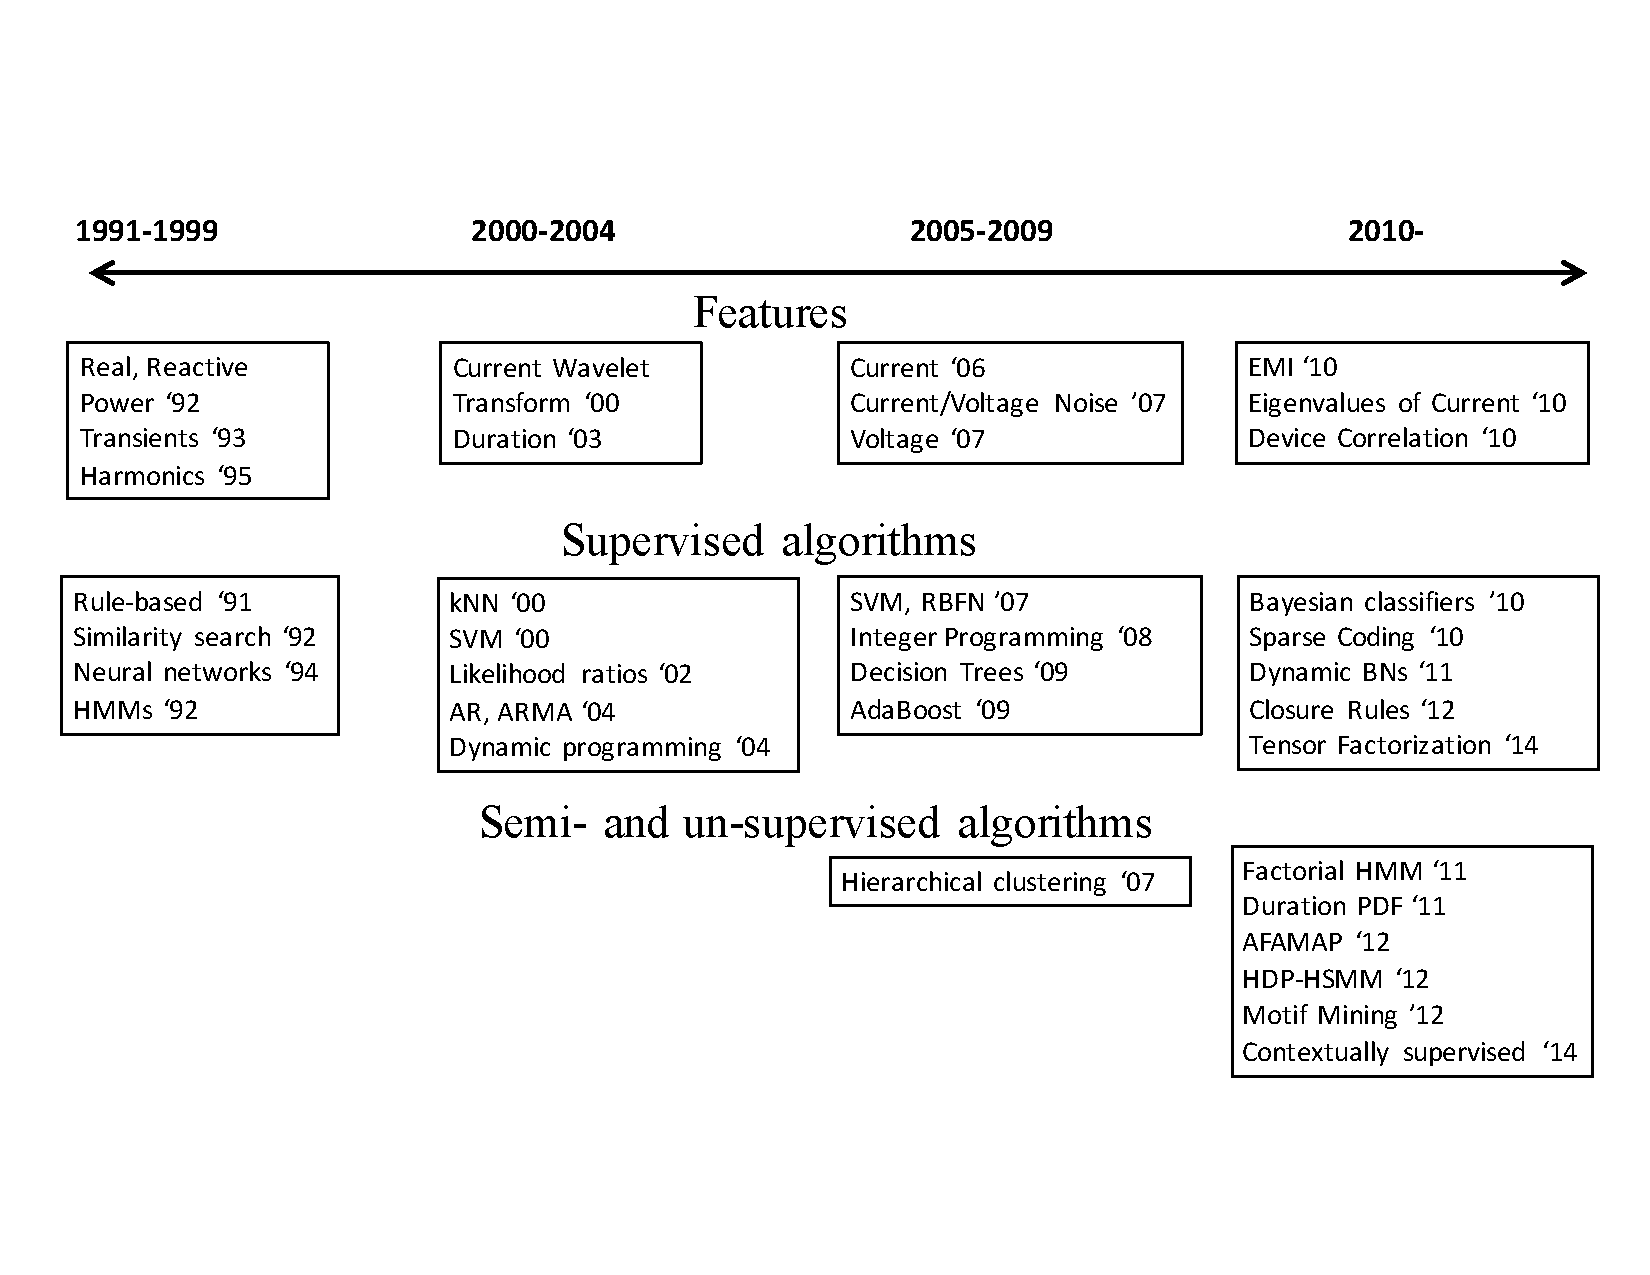
\includegraphics[width=5in]{figs/algo-timeline.pdf}
\caption{Timeline of features and algorithms proposed for energy disaggregation.}
\label{fig_timeline}
\end{figure}

Concomitantly,
algorithms adopted in this area have experienced an accelerating progress;
from supervised learning algorithms, including optimization algorithms 
and statistical models; 
to unsupervised learning and semi-supervised learning 
(see Fig.~\ref{fig_timeline}).
Supervised learning employs each circuit/device's data
as training data, which is laborious to collect.
%\manishc{what are the green ones?}\huijuanc{add the green ones' explanation.}
They include rule-based approaches; pair-wise matching
and neural  networks which were proposed in 1990s;
k-nearest neighbor algorithms (kNN); support vector machines (SVM) and kernel based
subspace classification (KSC); general likelihood ratio-based methods;
auto-regression and moving average methods; 
radial basis function network methods (RBFN);
decision trees; adaBoost; Bayesian classifiers;
space coding; dynamic Bayesian networks; closure rules;
Viterbi algorithms; dynamic programming, integer programming, 
and nonnegative tensor factorization.
%Also, the algorithm which is often employed in
%information processing area, wavelet transform,
%was used in 2000~\cite{chan2000harmonics}.
Since 2006, unsupervised and semi-supervised algorithms
have become the preferred approach to identify devices.
These include hierarchical clustering,
factorial HMMs, 
approximate factorial additive MAP (AFAMAP),
difference FHMM which adds prior knowledge of the device, 
hierarchical Dirichlet process hidden semi-Markov models,
motif mining, and contextually supervised source separation. 
In the next two sections, we explain the features and the algorithms in detail.




